\documentclass[12pt]{article}

\usepackage{sbc-template}
\usepackage{graphicx,url}
\usepackage[utf8]{inputenc}
\usepackage[brazil]{babel}
\usepackage{tabularx}
\usepackage{array}
\usepackage{ragged2e}
\usepackage{booktabs}
\usepackage{float}
\usepackage{makecell}

\sloppy

\title{Associação entre Precipitação e Gravidade dos Acidentes em Rodovias Federais no Estado de São Paulo}

\author{Gustavo Henrique Ferreira Alves\inst{1}, Gustavo Lima de Souza\inst{1}, Guilherme Padun Santos\inst{1}}

\address{ Escola de Artes, Ciências e Humanidades -- Universidade de São Paulo (EACH-USP)\\ São Paulo -- SP -- Brasil }

\begin{document} 

\maketitle

\begin{abstract}
This study investigates the association between precipitation and the severity
of traffic accidents on federal highways in the state of São Paulo. Accident
records from 2025 and the available records from 2026 from the Brazilian
Federal Highway Police (PRF) are integrated with precipitation measurements
from meteorological stations, considering spatial and temporal proximity.
Statistical analyses are used to evaluate whether precipitation levels are
associated with different levels of accident severity.
\end{abstract}

\begin{resumo}
Este trabalho investiga a associação entre a precipitação e a gravidade dos
acidentes em rodovias federais no estado de São Paulo. São utilizados registros
de acidentes da Polícia Rodoviária Federal (PRF) referentes a 2025 e aos dados
disponíveis de 2026, integrados a medições de precipitação provenientes de
estações meteorológicas, considerando a proximidade espacial e temporal entre
os registros. Por meio de análises estatísticas, será avaliado se diferentes
níveis de precipitação estão associados aos níveis de gravidade dos acidentes.
\end{resumo}

\section{Introdução}

Os acidentes de trânsito representam um importante problema de segurança viária e podem estar associados a fatores relacionados aos condutores, aos veículos, à infraestrutura das vias e às condições ambientais. No contexto das rodovias federais brasileiras, estudo realizado pela Fundação Dom Cabral (FDC), a partir de dados da Polícia Rodoviária Federal (PRF) e do Departamento Nacional de Infraestrutura de Transportes (DNIT), analisou 358.217 acidentes ocorridos entre 2018 e 2024, considerando rodovias com Volume Médio Diário Anual (VMDA) igual ou superior a 1.000 veículos. Entre as dimensões analisadas estão as condições meteorológicas e a taxa de severidade dos acidentes, evidenciando a relevância dessas variáveis para estudos de segurança rodoviária \cite{fdc2025}.

Entre os fatores ambientais, a precipitação merece atenção por modificar as condições de circulação e o comportamento do tráfego. Um estudo realizado com dados da BR-290, na região metropolitana de Porto Alegre, utilizou técnicas de agrupamento para caracterizar padrões de fluxo e velocidade associados a chuvas e acidentes \cite{caleffi2016}. Os resultados indicaram que períodos associados à ocorrência de chuva apresentaram redução de aproximadamente 10 km/h na velocidade dos veículos, evidenciando que condições meteorológicas adversas podem produzir alterações mensuráveis no comportamento do tráfego.

Entretanto, a relação entre precipitação e segurança viária não é necessariamente uniforme. Uma análise de séries históricas de acidentes com vítimas e variáveis meteorológicas realizada na França, nos Países Baixos e na região de Atenas identificou associações significativas entre condições meteorológicas e a ocorrência de acidentes \cite{bergel2013}. Entretanto, a magnitude e, em alguns casos, o sentido dessas relações variaram de acordo com a região e o tipo de via. Essa variabilidade reforça a importância de investigar o fenômeno em diferentes contextos geográficos e rodoviários.

No Brasil, a relação entre precipitação e acidentes foi investigada em um trecho da BR-376, no estado do Paraná, por meio da combinação de registros de acidentes e dados pluviométricos \cite{silva2020}. Por meio da Análise de Correspondência Múltipla, foram avaliadas associações entre características dos acidentes e dados de precipitação diária. Embora a intensidade da chuva não tenha apresentado associação significativa com as características dos acidentes analisados, a ocorrência de precipitação mostrou-se uma circunstância condicionante, indicando que a relação entre chuva e acidentes pode envolver fatores que vão além da quantidade de precipitação registrada.

Estudos recentes também demonstram a possibilidade de integrar registros de acidentes a informações meteorológicas provenientes de outras fontes. Em um estudo realizado em um trecho da BR-101, em Santa Catarina, registros de acidentes da PRF ocorridos entre 2017 e 2024 foram combinados com dados meteorológicos e de tráfego \cite{fuhr2026}. Embora o estudo tenha como objetivo a predição de acidentes, sua metodologia evidencia a viabilidade do enriquecimento dos registros da PRF com informações ambientais externas. Trabalhos recentes também têm investigado os efeitos da precipitação sobre a segurança rodoviária em escala nacional \cite{brasileiro2026}.

Os estudos encontrados abordam diferentes aspectos da relação entre precipitação e segurança viária, incluindo alterações no comportamento do tráfego, ocorrência de acidentes e características das ocorrências. Entretanto, permanece relevante investigar especificamente a associação entre a quantidade de precipitação registrada por estações meteorológicas e os diferentes níveis de gravidade dos acidentes. Nesse sentido, o estado de São Paulo constitui um recorte de interesse, permitindo relacionar registros georreferenciados de acidentes em rodovias federais a medições de precipitação espacial e temporalmente próximas às ocorrências. Essa abordagem possibilita utilizar a precipitação de forma quantitativa, em vez de considerar apenas a classificação qualitativa da condição meteorológica presente nos registros dos acidentes.

Dessa forma, este trabalho tem como objetivo \textbf{avaliar a associação entre a precipitação registrada por estações meteorológicas e a gravidade dos acidentes em rodovias federais no estado de São Paulo}. Para isso, pretende-se integrar registros de acidentes disponibilizados pela Polícia Rodoviária Federal a dados de precipitação provenientes de estações meteorológicas, considerando a proximidade espacial entre os locais dos acidentes e as estações, bem como a correspondência temporal entre as ocorrências e as medições de chuva.

\section{Trabalhos Correlatos}

A Tabela~\ref{tab:trabalhos_relacionados} sintetiza os principais estudos
abordados nesta seção, destacando os métodos empregados, os dados utilizados
e as principais diferenças em relação à abordagem adotada neste trabalho.

\begin{table}[H]
    \centering
    \caption{Comparação entre os trabalhos correlatos e a abordagem proposta.}
    \label{tab:trabalhos_relacionados}

    \footnotesize
    \renewcommand{\arraystretch}{1.35}
    \setlength{\tabcolsep}{3.5pt}

    \begin{tabularx}{\textwidth}{
        >{\RaggedRight\arraybackslash}p{2.7cm}
        >{\RaggedRight\arraybackslash}p{3.0cm}
        >{\RaggedRight\arraybackslash}p{3.7cm}
        >{\RaggedRight\arraybackslash}X
    }
        \toprule

        \textbf{Referência} &
        \textbf{Método} &
        \textbf{Dados utilizados} &
        \makecell[l]{\textbf{Diferencial deste}\\\textbf{trabalho}} \\

        \midrule

        \makecell[l]{Caleffi et al.\\(2016)} &
        K-means e Fuzzy C-Means &
        BR-290/RS; fluxo, velocidade, acidentes e clima &
        Analisa a associação entre precipitação e gravidade dos acidentes. \\

        \addlinespace

        \makecell[l]{Bergel-Hayat et al.\\(2013)} &
        Séries temporais &
        Acidentes e variáveis meteorológicas na Europa &
        Realiza análise específica das rodovias federais de São Paulo. \\

        \addlinespace

        \makecell[l]{Silva et al.\\(2020)} &
        Correspondência Múltipla &
        BR-376/PR; acidentes e precipitação diária &
        Utiliza precipitação horária associada espacial e temporalmente ao acidente. \\

        \addlinespace

        \makecell[l]{Fuhr e Inácio\\(2026)} &
        RF, SVM e MLP &
        BR-101/SC; PRF, meteorologia e tráfego &
        Avalia gravidade em vez de prever apenas a ocorrência de acidentes. \\

        \addlinespace

        \makecell[l]{Brasileiro et al.\\(2026)} &
        Heterogeneidade espacial &
        Acidentes e precipitação na malha federal brasileira &
        Adota recorte específico de São Paulo e três níveis de gravidade. \\

        \bottomrule
    \end{tabularx}
\end{table}

A relação entre condições meteorológicas e segurança viária tem sido investigada
por diferentes abordagens. Um estudo realizado na rodovia BR-290/RS analisou a
influência de condições climáticas e acidentes sobre o comportamento do tráfego
\cite{caleffi2016}. Foram integradas informações de fluxo, velocidade, acidentes
e condições meteorológicas, sendo identificadas alterações nas condições de
operação da rodovia durante períodos de chuva, incluindo redução da velocidade
dos veículos. O estudo evidencia que informações meteorológicas podem contribuir
para a caracterização das condições de circulação e segurança nas rodovias.

Mais diretamente relacionado à precipitação e às características dos acidentes,
um estudo realizado em um trecho da BR-376, no estado do Paraná, combinou
registros de acidentes e dados pluviométricos \cite{silva2020}. Por meio da
Análise de Correspondência Múltipla, foram avaliadas associações entre a
precipitação e diferentes características das ocorrências. Os resultados
indicaram que a intensidade da precipitação não apresentou associação
significativa com as características dos acidentes analisados, enquanto a
presença ou ausência de chuva se mostrou uma circunstância relevante. Esse
trabalho se aproxima da proposta deste estudo por relacionar diretamente
informações pluviométricas a características de acidentes rodoviários.

Em escala mais ampla, os efeitos da precipitação sobre a segurança nas rodovias
federais brasileiras foram investigados considerando diferenças de infraestrutura
e de contexto regional \cite{brasileiro2026}. Os resultados indicam que os efeitos
associados à chuva não são necessariamente uniformes em toda a malha rodoviária.
Esse resultado reforça a relevância de análises realizadas em recortes geográficos
específicos, como o estado de São Paulo.

Além da análise da relação entre precipitação e acidentes, estudos recentes
também demonstram a viabilidade da integração de diferentes fontes de dados.
Em um estudo realizado na BR-101, em Santa Catarina, registros da Polícia
Rodoviária Federal foram enriquecidos com informações meteorológicas e de
tráfego \cite{fuhr2026}. Embora o objetivo tenha sido a predição de acidentes
por meio de modelos de aprendizado de máquina, o trabalho é relevante para esta
pesquisa por demonstrar a utilização conjunta de dados da PRF e informações
meteorológicas externas.

Os estudos apresentados mostram que as condições meteorológicas podem estar
relacionadas a diferentes aspectos da segurança viária e que dados de acidentes
podem ser integrados a registros meteorológicos para investigar essas relações.
Entretanto, os trabalhos analisados diferem quanto ao recorte geográfico, às
variáveis consideradas e aos métodos empregados. Nesse contexto, este trabalho
se diferencia ao avaliar especificamente a associação entre a quantidade de
precipitação registrada por estações meteorológicas e os níveis de gravidade
dos acidentes em rodovias federais no estado de São Paulo.

\section{Metodologia}

A metodologia proposta está organizada em seis etapas principais: aquisição e preparação dos dados, integração espacial e temporal das bases, definição e tratamento das variáveis, análise descritiva, modelagem estatística e interpretação dos resultados.

Na primeira etapa, serão utilizados os registros de acidentes ocorridos em rodovias federais no estado de São Paulo, disponibilizados pela Polícia Rodoviária Federal (PRF) \cite{prf2026}. A base analisada compreenderá os acidentes registrados ao longo de 2025 e os registros disponíveis de 2026, atualmente correspondentes ao período entre 1º de janeiro e 31 de maio. A unidade de observação será o acidente rodoviário, de modo que cada linha do conjunto de dados resultante representará uma ocorrência. Entre as principais variáveis provenientes da PRF, serão consideradas \verb|id|, \verb|data_inversa|, \verb|horario|, \verb|br|, \verb|km|, \verb|municipio|, \verb|latitude|, \verb|longitude| e \verb|classificacao_acidente|. As variáveis \verb|mortos|, \verb|feridos_graves| e \verb|feridos_leves| poderão ser utilizadas de forma complementar para caracterizar a gravidade das ocorrências. Os registros de precipitação referentes aos períodos analisados serão obtidos a partir dos dados históricos das estações meteorológicas disponibilizados pelo Instituto Nacional de Meteorologia (INMET) \cite{inmet2026}.

Na segunda etapa, as bases da PRF e do INMET serão integradas por meio de correspondências espaciais e temporais. Para cada acidente, as coordenadas geográficas serão utilizadas para identificar uma estação meteorológica espacialmente próxima ao local da ocorrência. A data e o horário do acidente serão então relacionados aos registros da estação selecionada, permitindo associar uma medida quantitativa de precipitação, em milímetros, a cada ocorrência. Será estabelecido um limite máximo de distância entre o acidente e a estação meteorológica, bem como uma janela temporal para a associação das medições de precipitação. Esses critérios serão definidos com base na literatura e na distribuição espacial e temporal dos dados disponíveis. Estratégias semelhantes de integração entre informações de acidentes e dados meteorológicos têm sido empregadas em estudos anteriores \cite{silva2020,fuhr2026}.

Na terceira etapa, serão definidas e tratadas as variáveis utilizadas na análise. A variável de resposta será a gravidade do acidente, representada por \verb|classificacao_acidente| e organizada em três níveis ordenados: sem vítimas, com vítimas feridas e com vítimas fatais. A principal variável explicativa será a precipitação registrada pela estação meteorológica associada ao acidente, mantida inicialmente em sua forma quantitativa, em milímetros. Também serão tratados valores ausentes, inconsistências de formato e ocorrências para as quais não seja possível estabelecer uma correspondência meteorológica adequada.

Na quarta etapa, será realizada uma análise descritiva dos dados. Serão apresentadas as frequências e proporções das categorias de gravidade, bem como a distribuição dos valores de precipitação associados aos acidentes. Tabelas e representações gráficas serão utilizadas para comparar os níveis de gravidade em diferentes condições de precipitação e identificar padrões iniciais. De forma complementar, poderão ser construídas tabelas de contingência e aplicado o teste qui-quadrado de independência para uma análise exploratória da associação entre categorias de precipitação e gravidade.

Na quinta etapa, a associação entre precipitação e gravidade será avaliada por meio de Regressão Logística Ordinal. Inicialmente, será estimado um modelo contendo apenas a precipitação como variável explicativa, permitindo avaliar a associação bruta entre a quantidade de chuva e os níveis de gravidade dos acidentes. Em seguida, será estimado um modelo ajustado, incluindo características adicionais disponíveis na base da PRF, como fase do dia, tipo de pista e traçado da via, além das variáveis temporais ano e mês, com o objetivo de verificar se a associação observada para a precipitação permanece após a consideração de outros fatores relacionados às ocorrências.

Os resultados dos modelos serão avaliados a partir dos coeficientes estimados, razões de chances (\textit{odds ratios}), intervalos de confiança e níveis de significância estatística. Também será verificada a adequação da hipótese de chances proporcionais, necessária à Regressão Logística Ordinal. Caso essa hipótese não seja considerada adequada aos dados, será avaliada a utilização de um modelo alternativo, como a Regressão Logística Multinomial.

Por fim, na sexta etapa, os resultados serão interpretados com o objetivo de determinar a direção e a magnitude da associação entre precipitação e gravidade dos acidentes. A análise permitirá avaliar se aumentos na quantidade de precipitação estão associados a maiores ou menores chances de ocorrência em categorias mais elevadas de gravidade, tanto de forma isolada quanto após o ajuste por outras características das ocorrências. Também serão consideradas as limitações relacionadas à distância entre acidentes e estações meteorológicas, à resolução temporal das medições e às possíveis perdas de registros durante a integração das bases.

\section{Cronograma}\label{sec:cronograma}

\begin{table}[H]    
\centering
    \caption{Cronograma das atividades}
    \label{tab:cronograma}

    \small
    \renewcommand{\arraystretch}{1.25}
    \setlength{\tabcolsep}{4pt}

    \begin{tabularx}{\textwidth}{
        >{\RaggedRight\arraybackslash}X
        >{\centering\arraybackslash}p{1.7cm}
        >{\centering\arraybackslash}p{1.7cm}
        >{\centering\arraybackslash}p{1.7cm}
    }
        \toprule

        \textbf{Atividade} &
        \textbf{Setembro} &
        \textbf{Outubro} &
        \textbf{Novembro} \\

        \midrule

        Aquisição e preparação dos dados
        & \textbf{X} & & \\

        Integração espacial e temporal PRF--INMET
        & \textbf{X} & \textbf{X} & \\

        Definição e tratamento das variáveis
        & \textbf{X} & \textbf{X} & \\

        Análise descritiva dos dados
        & \textbf{X} & \textbf{X} & \\

        Modelagem estatística
        & & \textbf{X} & \textbf{X} \\

        Avaliação e diagnóstico dos modelos
        & & \textbf{X} & \textbf{X} \\

        Análises de sensibilidade
        & & \textbf{X} & \textbf{X} \\

        Análise e interpretação dos resultados
        & & \textbf{X} & \textbf{X} \\

        Redação e revisão do trabalho
        & & \textbf{X} & \textbf{X} \\

        \bottomrule
    \end{tabularx}
\end{table}
\section{Resultados preliminares}
\label{sec:resultados}

A preparação das bases da Polícia Rodoviária Federal (PRF) resultou em
6.515 acidentes ocorridos em rodovias federais no estado de São Paulo.
Desse total, 4.683 correspondem a ocorrências registradas ao longo de 2025
e 1.832 a ocorrências registradas entre 1º de janeiro e 31 de maio de 2026,
período disponível na base utilizada. Entre os acidentes analisados,
5.273 foram classificados como acidentes com vítimas feridas, 971 como
acidentes sem vítimas e 271 como acidentes com vítimas fatais.

Para os dados meteorológicos, foram consideradas 40 estações automáticas
do Instituto Nacional de Meteorologia (INMET) localizadas no estado de
São Paulo, totalizando 583.680 registros horários. Cada acidente foi
associado inicialmente à estação meteorológica geograficamente mais próxima
e, posteriormente, à medição temporalmente mais próxima de seu horário.

Dos 6.515 acidentes, 5.661 apresentaram valor válido de precipitação na
medição associada, enquanto 854 apresentaram valor ausente para essa
variável, correspondendo a aproximadamente 13,1\% da base. A diferença
temporal média entre o horário do acidente e a medição selecionada foi de
14,8 minutos, com mediana de 15 minutos. O primeiro e o terceiro quartis
foram de aproximadamente 6 e 20 minutos, respectivamente, e a maior
diferença observada foi de 30 minutos.

Em relação à correspondência espacial, a distância média entre os acidentes
e as respectivas estações meteorológicas foi de aproximadamente 26,2 km,
com mediana de 21,7 km. O primeiro e o terceiro quartis foram de 12,1 km
e 39,2 km, respectivamente, e a maior distância observada foi de 81,8 km.
A Figura~\ref{fig:distancia_estacoes} apresenta a distribuição dessas
distâncias.

\begin{figure}[htbp]
    \centering
    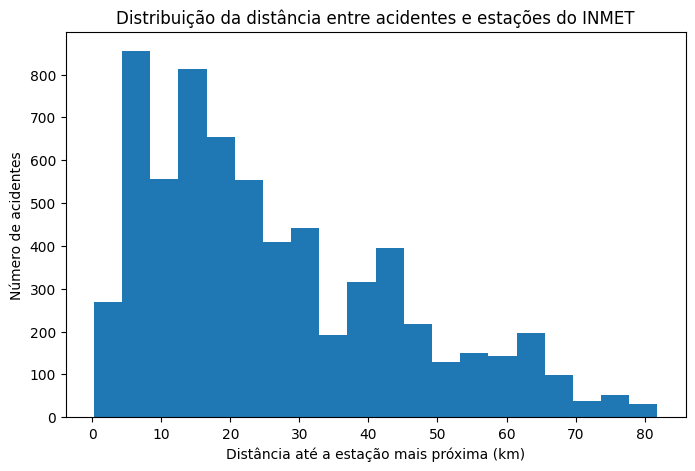
\includegraphics[width=0.72\linewidth]{distancia_estacoes.png}
    \caption{Distribuição da distância entre os acidentes e as estações meteorológicas do INMET.}
    \label{fig:distancia_estacoes}
\end{figure}

Observa-se maior concentração de ocorrências associadas a estações
relativamente próximas, embora também existam acidentes associados a
estações mais distantes. Essa característica foi considerada na definição
do limite espacial utilizado para a composição da base de modelagem.

Entre os 5.661 acidentes com medição válida, a precipitação média foi de
aproximadamente 0,24 mm, com valor máximo de 82,0 mm. O primeiro quartil,
a mediana e o terceiro quartil foram iguais a zero, evidenciando forte
concentração de registros sem precipitação. Apenas 559 acidentes,
aproximadamente 9,9\% das ocorrências com medição válida, apresentaram
precipitação superior a zero.

De forma exploratória, a precipitação média associada aos acidentes com
vítimas fatais foi de aproximadamente 0,25 mm. Para os acidentes com vítimas
feridas, a média foi de aproximadamente 0,21 mm, enquanto para os acidentes
sem vítimas foi de aproximadamente 0,42 mm. Essas médias devem ser
interpretadas com cautela devido à forte concentração de valores iguais
a zero e à presença de valores elevados.

A Figura~\ref{fig:chuva_gravidade} apresenta o percentual de acidentes com
precipitação superior a zero em cada categoria de gravidade, permitindo
comparar a frequência relativa de registros de chuva sem depender apenas
das médias de precipitação.

\begin{figure}[htbp]
    \centering
    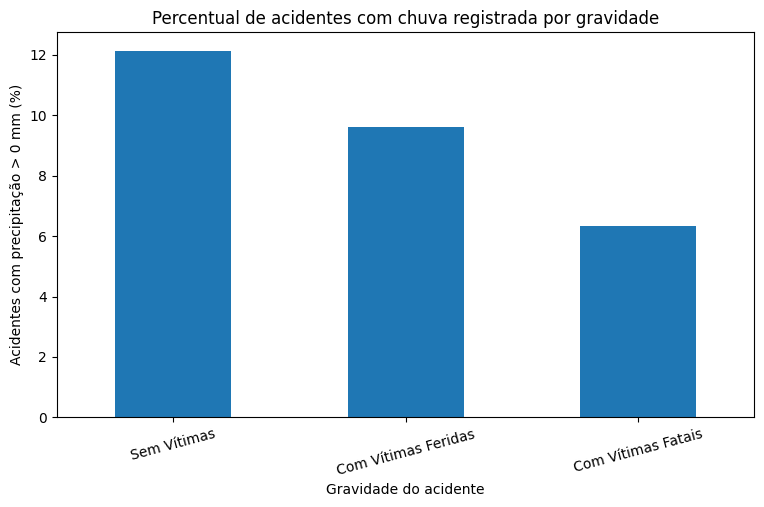
\includegraphics[width=0.72\linewidth]{chuva_gravidade.png}
    \caption{Percentual de acidentes com precipitação superior a zero segundo a gravidade da ocorrência.}
    \label{fig:chuva_gravidade}
\end{figure}

Também foi investigado o padrão dos 854 registros com precipitação ausente.
Após ajuste por gravidade, ano, mês, distância até a estação, condição
meteorológica registrada pela PRF e estação do INMET, não foi identificada
associação estatisticamente significativa entre gravidade e ausência da
medição. Em relação aos acidentes fatais, foram obtidos $p = 0,155$ para
acidentes com vítimas feridas e $p = 0,765$ para acidentes sem vítimas.

Embora esse resultado não permita afirmar que os dados ausentes sejam
completamente aleatórios, ele torna mais defensável a utilização de casos
completos na análise principal. A presença de medições ausentes permanece,
entretanto, como uma limitação do estudo.

Para a modelagem principal, foi adotado um limite máximo de 30 km entre o
local do acidente e a estação meteorológica. Dos 5.661 acidentes com
precipitação válida, 1.931 foram excluídos por apresentarem distância
superior a esse limite. Como a maior diferença temporal observada foi de
30 minutos, nenhum registro adicional foi excluído pelo critério temporal
de até 60 minutos.

A base final de modelagem foi composta por 3.730 acidentes, correspondendo
a aproximadamente 57,3\% dos 6.515 acidentes inicialmente considerados.
Desse total, 3.058 foram classificados como acidentes com vítimas feridas,
530 como acidentes sem vítimas e 142 como acidentes com vítimas fatais.
Entre essas ocorrências, 402, aproximadamente 10,8\%, apresentaram
precipitação superior a zero.

Cabe destacar que a principal redução da amostra ocorreu devido ao critério
espacial de 30 km. Embora esse limite aumente a proximidade entre o local
do acidente e a medição utilizada para representar a condição meteorológica,
ele também reduz o número de observações disponíveis. Por esse motivo,
limites de 40 km e 50 km foram posteriormente avaliados em análises de
sensibilidade.

A associação entre precipitação e gravidade foi inicialmente avaliada por
meio de Regressão Logística Ordinal, considerando a ordem das três categorias
da variável de resposta: sem vítimas, com vítimas feridas e com vítimas
fatais. Foram estimados modelos brutos, contendo apenas a precipitação, e
modelos ajustados por fase do dia, tipo de pista, traçado da via, ano e mês.

A precipitação foi analisada tanto como variável contínua, expressa em
milímetros, quanto de forma binária, diferenciando situações com e sem
precipitação registrada.

Os resultados foram interpretados a partir da razão de chances
(\textit{odds ratio} -- OR), do intervalo de confiança de 95\% (IC95\%)
e do valor de $p$. Valores de OR superiores a 1 indicam aumento das chances,
enquanto valores inferiores a 1 indicam redução. Para a precipitação
contínua, a OR representa a variação associada ao aumento de 1 mm.
Foi adotado $p < 0,05$ como critério de significância estatística; quando
o IC95\% inclui o valor 1, não há evidência estatística suficiente de que
a OR difira de 1 ao nível de 5\%.

No modelo ordinal bruto com precipitação contínua, foi obtida OR = 0,978
e $p = 0,124$. Após o ajuste pelas demais variáveis, a estimativa permaneceu
semelhante, com OR = 0,977
(IC95\%: 0,949--1,006; $p = 0,123$).

A OR de 0,977 corresponde a uma estimativa de redução de aproximadamente
2,3\% nas chances de o acidente pertencer a uma categoria mais elevada de
gravidade para cada aumento de 1 mm de precipitação. Entretanto, como o
intervalo de confiança inclui o valor 1 e o valor de $p$ é superior a 0,05,
não foi encontrada evidência estatisticamente significativa dessa associação.

Para a variável binária de chuva, o modelo bruto apresentou OR = 0,766 e
$p = 0,042$. Entretanto, após o ajuste por fase do dia, tipo de pista,
traçado da via, ano e mês, foi obtida OR = 0,831
(IC95\%: 0,638--1,084; $p = 0,172$). Assim, a associação observada no
modelo bruto não permaneceu estatisticamente significativa após o ajuste,
indicando que parte desse resultado pode estar relacionada às demais
características consideradas no modelo.

A Tabela~\ref{tab:modelos_principais} apresenta os principais resultados
dos modelos ajustados.

\begin{table}[htbp]
    \centering
    \caption{Resultados dos modelos ajustados para precipitação.}
    \label{tab:modelos_principais}
    \footnotesize
    \renewcommand{\arraystretch}{1.1}
    \setlength{\tabcolsep}{3pt}

    \begin{tabularx}{\textwidth}{
        >{\RaggedRight\arraybackslash}X
        >{\centering\arraybackslash}p{1.1cm}
        >{\centering\arraybackslash}p{2.0cm}
        >{\centering\arraybackslash}p{1.1cm}
    }
        \toprule
        \textbf{Modelo} &
        \textbf{OR} &
        \textbf{IC95\%} &
        \textbf{$p$} \\
        \midrule

        Ordinal -- precipitação (mm) &
        0,977 & 0,949--1,006 & 0,123 \\

        Ordinal -- chuva binária &
        0,831 & 0,638--1,084 & 0,172 \\

        Multinomial -- feridos vs. sem vítimas (mm) &
        0,973 & 0,944--1,003 & 0,075 \\

        Multinomial -- fatais vs. sem vítimas (mm) &
        0,989 & 0,924--1,058 & 0,744 \\

        Multinomial -- feridos vs. sem vítimas (chuva) &
        0,899 & 0,672--1,204 & 0,474 \\

        Multinomial -- fatais vs. sem vítimas (chuva) &
        0,554 & 0,265--1,159 & 0,117 \\

        \bottomrule
    \end{tabularx}
\end{table}

A hipótese de chances proporcionais da Regressão Logística Ordinal também
foi avaliada de forma exploratória. Para a precipitação contínua, foram
obtidas OR = 0,974 ($p = 0,079$) e OR = 1,009 ($p = 0,786$) nos dois
pontos de corte analisados, além de diferenças nos coeficientes de algumas
covariáveis. Embora esse procedimento não constitua um teste formal da
hipótese, os resultados motivaram a utilização da Regressão Logística
Multinomial como análise complementar.

No modelo multinomial, os acidentes sem vítimas foram utilizados como
categoria de referência. Para a precipitação contínua, foram obtidas
OR = 0,973 (IC95\%: 0,944--1,003; $p = 0,075$) para acidentes com vítimas
feridas e OR = 0,989 (IC95\%: 0,924--1,058; $p = 0,744$) para acidentes
fatais. Para a variável binária, as estimativas foram OR = 0,899
(IC95\%: 0,672--1,204; $p = 0,474$) e OR = 0,554
(IC95\%: 0,265--1,159; $p = 0,117$), respectivamente.

Como todos os intervalos de confiança incluíram o valor 1 e os valores de
$p$ foram superiores a 0,05, a análise multinomial também não apresentou
evidência estatisticamente significativa de associação entre precipitação
e gravidade.

Também foi realizada uma análise de sensibilidade em relação ao limite
espacial utilizado para associar os acidentes às estações meteorológicas.
Além do limite principal de 30 km, foram considerados limites de 40 km e
50 km, resultando em amostras de 3.730, 4.339 e 5.015 acidentes,
respectivamente.

Para a precipitação contínua, as estimativas permaneceram semelhantes:
OR = 0,977 para 30 km, OR = 0,978 para 40 km e OR = 0,976 para 50 km.
Os respectivos valores de $p$ foram 0,123, 0,127 e 0,082, permanecendo
acima do nível de significância de 5\%.

Para a variável binária, observou-se maior sensibilidade ao limite espacial.
Foram obtidas OR = 0,831 ($p = 0,172$) para 30 km,
OR = 0,788 ($p = 0,058$) para 40 km e
OR = 0,775 ($p = 0,032$) para 50 km.

O resultado significativo observado com 50 km não foi utilizado para
redefinir a análise principal, pois os limites adicionais foram empregados
como análise de sensibilidade e não como critério para selecionar resultados
com base no valor de $p$. Dessa forma, o limite de 30 km foi mantido como
referência principal.

De forma geral, os modelos ajustados da análise principal não forneceram
evidência estatisticamente significativa de associação entre precipitação
e gravidade dos acidentes. A conclusão foi semelhante nos modelos ordinal
e multinomial para a precipitação contínua, enquanto a representação binária
mostrou maior sensibilidade ao limite espacial adotado.

Esses resultados representam ausência de evidência estatística suficiente
de associação nos dados e critérios analisados, e não evidência de ausência
de qualquer efeito da precipitação. Entre as principais limitações estão a
cobertura espacial das estações meteorológicas, a redução da amostra pelo
limite de 30 km, a elevada concentração de registros sem precipitação e a
presença de medições ausentes.
\section{Conclusão}
\label{sec:conclusao}

Este trabalho avaliou a associação entre a precipitação registrada por
estações meteorológicas e a gravidade dos acidentes ocorridos em rodovias
federais no estado de São Paulo. A integração entre os registros da Polícia
Rodoviária Federal e as medições horárias do INMET mostrou-se viável, com
5.661 dos 6.515 acidentes apresentando uma medição válida de precipitação
associada.

Para a análise principal, foi adotado um limite máximo de 30 km entre o
local do acidente e a estação meteorológica, resultando em uma base final
de 3.730 ocorrências. A precipitação foi analisada tanto de forma contínua,
em milímetros, quanto de forma binária, distinguindo situações com e sem
registro de chuva.

Nos modelos de Regressão Logística Ordinal ajustados por fase do dia, tipo
de pista, traçado da via, ano e mês, não foi encontrada evidência
estatisticamente significativa de associação entre precipitação e maiores
níveis de gravidade dos acidentes. Para a precipitação contínua, foi obtida
OR = 0,977 (IC95\%: 0,949-1,006; $p = 0,123$), enquanto para a variável
binária de chuva foi obtida OR = 0,831 (IC95\%: 0,638-1,084; $p = 0,172$).

Como análise de sensibilidade, também foi ajustado um modelo de Regressão
Logística Multinomial, que apresentou conclusão semelhante. A precipitação
não mostrou associação estatisticamente significativa nem na comparação
entre acidentes com vítimas feridas e acidentes sem vítimas, nem na
comparação entre acidentes fatais e acidentes sem vítimas. A análise de
sensibilidade espacial também indicou que os resultados para precipitação
contínua permaneceram estáveis nos limites de 30, 40 e 50 km, enquanto a
representação binária da chuva apresentou maior sensibilidade ao critério
de distância adotado.

Os resultados devem ser interpretados considerando algumas limitações,
entre elas a presença de medições meteorológicas ausentes, a dependência
da proximidade entre acidente e estação, a concentração elevada de
observações sem precipitação e a utilização apenas de estações localizadas
no estado de São Paulo. Além disso, o estudo avalia a gravidade entre os
acidentes observados e não o risco de ocorrência de acidentes em situações
com ou sem chuva.

Dessa forma, considerando os dados e os critérios adotados, não foi
encontrada evidência estatisticamente significativa de associação entre
a quantidade de precipitação e a gravidade dos acidentes na análise
principal. Os resultados reforçam, contudo, a importância de considerar
a qualidade da integração espacial e temporal entre bases de acidentes e
dados meteorológicos em estudos dessa natureza.

\bibliographystyle{sbc}
\bibliography{sbc-template}

\end{document}